\subsection{State Feedback with Integral Control}
The aim of the attitude controller is to be able to track the references for roll, pitch and yaw. Given a state space representation as the one in \autoref{xDotLinear} and \ref{yLinear}, it is possible to design an attitude controller so that this aim is achieved. %the dynamics of the system can be chosen.

In this approach, a state feedback is used to make the system return to the equilibrium position while an integral controller makes it possible to include a new reference and track it while rejecting input disturbances. These two control actions are added together and four velocity values for the motors are transmitted to the Rotational Speed Calculator seen in \autoref{fig:ControlHeadDiagram}. The diagram in \autoref{fig:ControllerColorDiagram} shows how the two controllers are related. The \autoref{fig:DetailedControllerColorDiagram} illustrates the highlighted part in \autoref{fig:ControllerColorDiagram} in more detail, with the actual variables used in the design process.
%
%In this approach a state feedback is used to allow the system to return to equilibrium position while an integral controller makes it possible to include a new reference and track it, adding both control actions to get the one finally applied to the motors.
\begin{minipage}{\linewidth}
	\begin{minipage}{0.5\linewidth}
		\begin{figure}[H]
			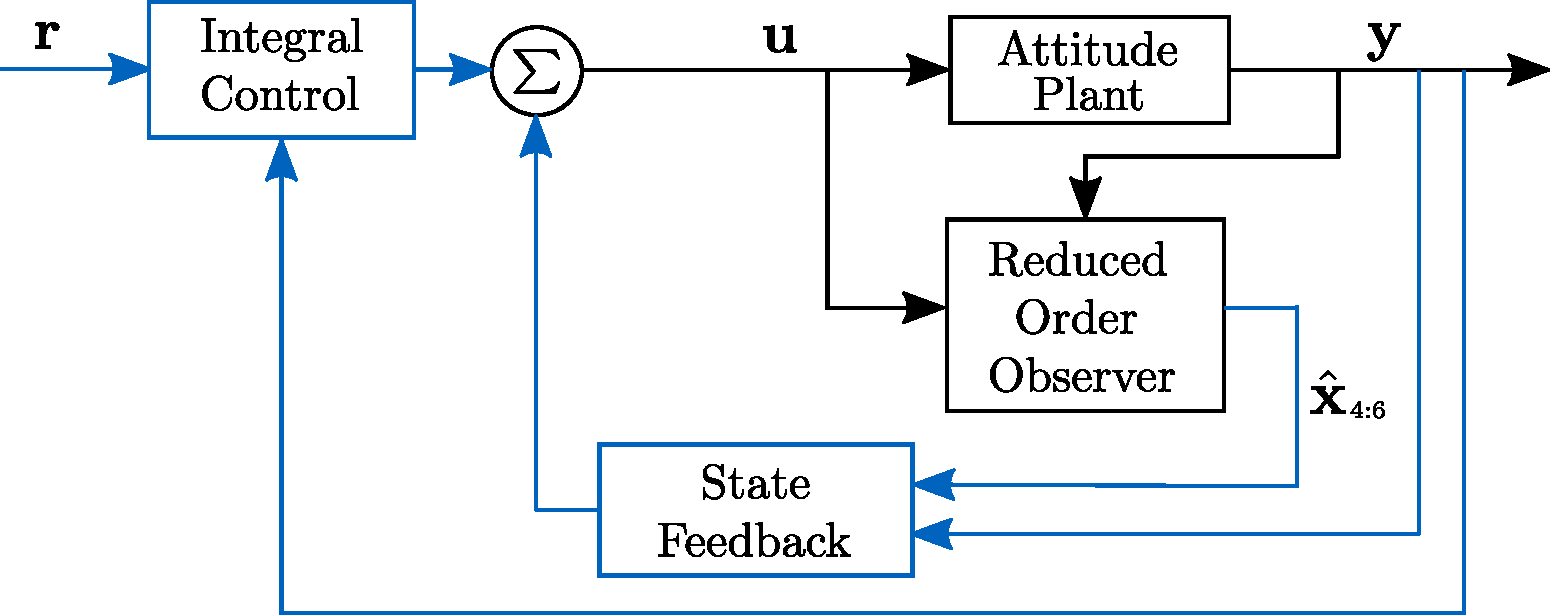
\includegraphics[scale=.35]{figures/ControllerColorDiagram}
			\centering			
			\captionof{figure}{Control structure highlighting the state feedback and integral control.}
			\label{fig:ControllerColorDiagram}
		\end{figure}
	\end{minipage}
	\hspace{0.03\linewidth}
	\begin{minipage}{0.5\linewidth}
		\begin{figure}[H]%\vspace{20mm}
			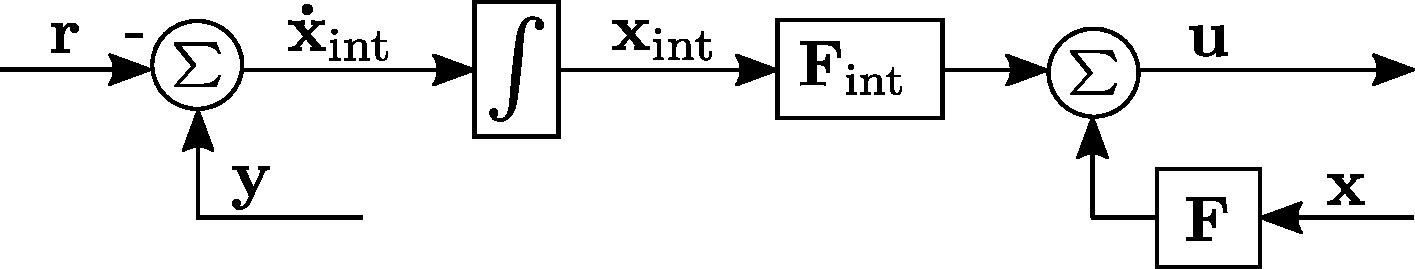
\includegraphics[scale=.3]{figures/DetailedControllerColorDiagram}
			\centering %\vspace{7mm}
			\captionof{figure}{The highlighted parts from the left diagram in detail, including all the variables used in the design of the controller.}
			\label{fig:DetailedControllerColorDiagram}
		\end{figure}
	\end{minipage}
\end{minipage}


From \autoref{fig:DetailedControllerColorDiagram}, the feedback law yields \autoref{eq:ssControllerAction}.
%
\begin{flalign} 
	\vec{u} &=\vec{F}  \vec{x} + \vec{F}_{\mathrm{Int}}  \vec{x}_{\mathrm{Int}}
     \label{eq:ssControllerAction}
\end{flalign}
%
\begin{where}
	\va{\vec{F}}{is a 4x6 state feedback matrix}{}
	\va{\vec{F}_{\mathrm{Int}}}{is a 3x6 integral feedback matrix }{}
\end{where}

In this equation, \si{\vec{x}_{\mathrm{Int}}} is given by \autoref{eq:ssControllerAction1}, which is equivalent to \autoref{eq:ssControllerAction2}, see \autoref{fig:DetailedControllerColorDiagram}.
\begin{flalign}
    \vec{x}_{\mathrm{Int}} &= \int_{0}^{t} \vec{y}(\tau)-\vec{r}(\tau) \ d\tau	\label{eq:ssControllerAction1}\\
    \vec{\dot{x}}_{\mathrm{Int}} &= \vec{y}-\vec{r} \label{eq:ssControllerAction2}
\end{flalign} 
%
This last equation is included in the existing state space model, having the system states, $\vec{x}$, and taking \si{\vec{x}_{\mathrm{Int}}} as new states, yielding the expressions \autoref{xdotSSExtended} and \ref{ySSExtended} \cite{ssReference}.
%
\begin{flalign} 
    \dot{\vec{x}}_{\mathrm{e}} &= \vec{A}_{\mathrm{e}}  \vec{x}_{\mathrm{e}} + \vec{B}_{\mathrm{e}}  \vec{u} + 
    \begin{bmatrix}
       \ \vec{0}     \ \ \ \\ 
       \ \vec{-I}     \ \ \  		
   \end{bmatrix}
   \vec{r} 
   \label{xdotSSExtended}\\ 
    \vec{y} &= \vec{C}_{\mathrm{e}}  \vec{x}_{\mathrm{e}} 
       \label{ySSExtended}
\end{flalign} 
%
where\\
\begin{minipage}{0.24\linewidth}
	\begin{flalign}
		\dot{\vec{x}}_{\mathrm{e}}= 
		\begin{bmatrix}
			\ \dot{\vec{x}}      \ \ \ \\ 
			\ \dot{\vec{x}}_{\mathrm{Int}}      \ \ \  		
		\end{bmatrix} \nonumber
	\end{flalign}
\end{minipage}\hfill
\begin{minipage}{0.24\linewidth}
	\begin{flalign}
	    \vec{A}_{\mathrm{e}}=
	    \begin{bmatrix}
	        \ \vec{A}  & \vec{0}    \ \ \ \\ 
	        \ \vec{C}  & \vec{0}    \ \ \  		
	    \end{bmatrix} \nonumber
	\end{flalign}
\end{minipage}   \hfill 
\begin{minipage}{0.24\linewidth}
	\begin{flalign}
		\vec{B}_{\mathrm{e}}=
		\begin{bmatrix}
			\ \vec{B}    \ \ \ \\ 
			\ \vec{0}     \ \ \  		
		\end{bmatrix} \nonumber
	\end{flalign}
\end{minipage}\hfill
\begin{minipage}{0.24\linewidth}
	\begin{flalign}
		\vec{C}_{\mathrm{e}}=
		\begin{bmatrix}
			\ \vec{C}  & \vec{0}  \ \ \  		
		\end{bmatrix} \nonumber
	\end{flalign}
\end{minipage}

The resulting feedback law can be design as a conventional state feedback, where the goal is to choose an appropriate $\vec{F}_{\mathrm{e}}=[\vec{F} \ \vec{F}_{\mathrm{Int}}]$ matrix such that the eigenvalues of $\vec{A}_{\mathrm{e}}+\vec{B}_{\mathrm{e}}\vec{F}_{\mathrm{e}}$ are the new poles of the system.




